\documentclass[12pt, a4paper]{article}
\usepackage{amsmath, amssymb, amsthm, graphicx}
\usepackage{mathrsfs}
\usepackage{listings}

\lstset{basicstyle=\ttfamily}
\usepackage[numbered]{mcode}



\newcommand{\dx}{\,{\rm d}x}
\newcommand{\dd}{\,{\rm d}}
\newcommand{\deq}{\stackrel{\rm def}{=}}
\newcommand{\mbb}{\mathbb}
\newcommand{\mbf}{\bs}
\newcommand{\bs}{\boldsymbol}
\newcommand{\mcal}{\mathcal}
\newcommand{\mc}{\mcode}
\newcommand{\lla}{\langle}
\newcommand{\rra}{\rangle}
\newcommand{\supp}{\operatorname{supp}}
\newcommand{\range}{\operatorname{range}}
\newcommand{\PartSize}{\fontsize{0.85cm}{0.85cm}\selectfont} 
\newcommand{\mscr}{\mathscr}

\newcommand{\curl}{{\rm curl\,}}
\renewcommand{\div}{\operatorname{div}}
\newcommand{\tr}{\operatorname{tr}}
\newcommand{\dev}{\operatorname{dev}}
\newcommand{\sym}{\operatorname{sym}}
\newcommand{\skw}{\operatorname{skw}}
\newcommand{\spn}{\operatorname{spn}}
\newcommand{\mspn}{\operatorname{mspn}}
\newcommand{\vspn}{\operatorname{vspn}}
\newcommand{\mskw}{\operatorname{mskw}}
\newcommand{\vskw}{\operatorname{vskw}}
\newcommand{\defm}{\operatorname{def}}
\newcommand{\hess}{\operatorname{hess}}
\newcommand{\inc}{\operatorname{inc}}
\newcommand{\dex}{\operatorname{dex}}


\newtheorem{theorem}{Theorem}
\newtheorem{corollary}{Corollary}
\newtheorem{lemma}{Lemma}
\newtheorem{remark}[theorem]{Remark}


\begin{document}

\section{Introduction}

The expansive world of finite element methods (FEM) has been constantly
evolving, offering innovative approaches to complex computational problems in
areas such as electromagnetism and fluid dynamics. Within this landscape, the
H(curl) and H(div) conforming finite elements, epitomized by the BDM and Nédélec
elements, have proven indispensable in advancing computational electromagnetism.

Over the past decades, finite element methods (FEM) have garnered significant
attention due to their versatility and efficiency in solving a plethora of
computational problems, particularly in the realms of electromagnetics and fluid
dynamics. The H(curl) and H(div) conforming finite elements, epitomized by BDM
and Nédélec elements, serve as quintessential examples of this exploration,
offering profound insights into computational electromagnetism.

One foundational work in the area is Arnold, Falk, and Winther's research on
Finite Element Exterior Calculus (FEEC) \cite{ArnoldFalkWinther2006}, which
charted a structured path towards understanding finite element discretizations.
This was subsequently built upon in studies such as geometric decompositions by
Arnold, Falk, and Winther \cite{ArnoldFalkWinther2009}, the high-order finite
element spaces insights by Christiansen and Rapetti
\cite{ChristiansenRapetti2016}, the focus on boundary degrees of freedom by Chen
and Huang \cite{Chen;Huang:2021Geometric}, and the exploration of discontinuous
nodal finite elements by Hu, Hu, and Zhang \cite{HuHuZhang2022}.

Recently, Rognes, Kirby, and Logg \cite{RognesKirbyLogg2010} brought a paradigm
shift by proposing an efficient evaluation and assembly mechanism for finite
element variational forms on \( H(curl) \) and \( H(div) \). Their approach
leverages a decomposition of the element tensor into a precomputable reference
tensor and a mesh-dependent geometry tensor. Importantly, they innovatively
tackled challenges related to the mapping of basis functions and the orientation
of geometrical entities. Such advancements facilitate an automated and
user-friendly implementation that allows specification of finite element
variational forms in almost mathematical notation, ushering in newfound
efficiencies in the field.

Motivated by these preceding works, our study seeks to delve deeper into the
intricacies of basis functions for BDM and Nédélec elements. We draw from the
concepts of partially discontinuous nodal elements and the efficient assembly
techniques proposed by Rognes, Kirby, and Logg. Ensuring trace continuity will
be our primary focus, given its paramount importance for the stability and
accuracy of numerical solutions.

Our paper structure is as follows: Section 2 will elucidate foundational
concepts such as simplicial lattices, interpolation points, bubble polynomials,
and triangulation. Sections 3, 4, and 5 will delve into Lagrange, BDM, and
Nédélec elements, enriched with insights from the innovative assembly
methodologies. Section 6 will address the degrees of freedom, vital for
effective matrix assembly.  Section 7 presents two numerical examples, which solve the mixed Poisson
problem and Maxwell problem using BDM and second kind Nédélec elements,
respectively, to verify the correctness of the basis function construction.


\section{Preliminaries}

\subsection{Simplicial Lattice}

A simplicial lattice is characterized by multi-indices, $\boldsymbol\alpha$, with a length
of $n+1$ where each component is a non-negative integer. The degree of a
multi-index is the sum of its components. We denote the set of all multi-indices of
degree $k$ as $\mathbb T^n_k$. Multi-indices can be arranged using the dictionary order, \(R_n\),
which depends on the length of the multi-index.

\subsection{Interpolation Points}

An \(n\)-simplex, \(T\), is defined by the convex hull of \(n+1\) distinct points.
Every point within \(T\) can be expressed using barycentric coordinates, \(\bs\lambda\).
The set \(\mathbb T^n_k\) of multi-indices can be embedded geometrically into \(T\).
Their ordering is described by \(R_n(\bs\alpha)\). The figure 
showcases the interpolation points on a triangle for the degree \(k=4\).

\subsection{Sub-simplices and Sub-simplicial Lattices}

Any simplex, \(T\), encompasses subsimplices across multiple dimensions.
\(\Delta(T)\) encompasses all subsimplices within \(T\), while \(\Delta_{\ell}(T)\)
focuses on those of dimension \(\ell\). Each sub-simplex has both geometric and algebraic
representations. Additionally, for each sub-simplex \(f\), there is a corresponding
opposite sub-simplex \(f^*\). The relationship between a multi-index in a sub-simplex
and its encompassing simplex is outlined by the prolongation/extension operator, \(E\).


\subsection{Bubble Polynomial}
The Bernstein representation defines the polynomial space of degree \(k\) over a
simplex. A sub-simplex, \(f\), has its bubble polynomial, which is of 
degree \(\ell + 1\). This bubble polynomial exhibits properties that make it zero on specific subsimplices.

\subsection{Triangulation}
A geometric triangulation of a polyhedral domain, \(\Omega\), in \(\mathbb R^n\)
consists of \(n\)-simplices. 


\section{Geometric Decompositions of Lagrange elements}

\subsection{Geometric decomposition}

For the polynomial space $\mathbb P_k(T)$ with $k\geq 1$ on an $n$-dimensional simplex $T$, we have the following geometric decomposition of Lagrange element:

\begin{theorem}[Geometric decomposition of Lagrange element]
\label{thm:Lagrangedec}
For the polynomial space $\mathbb P_k(T)$ with $k\geq 1$ on an $n$-dimensional simplex $T$, the decomposition is given by:
\begin{align}
\mathbb P_k(T) &= \bigoplus_{\ell = 0}^n \bigoplus_{f\in \Delta_{\ell}(T)} b_f\mathbb P_{k - (\ell +1)} (f).
\end{align}
\end{theorem}

Furthermore, the bubble polynomial space of degree $k$ on a sub-simplex $f$ is defined by:
$$
\mathbb B_{k}( f) := b_f\mathbb P_{k - (\ell +1)} (f).
$$

Thus, we can rewrite the decomposition as:
\begin{equation}
\mathbb P_k(T) = \mathbb P_1(T) \oplus \bigoplus_{\ell = 1}^n \bigoplus_{f\in \Delta_{\ell}(T)} \mathbb B_{k}( f).
\end{equation}

\subsection{Lagrange interpolation basis functions}

We can represent the DoFs as function values on the interpolation points:

\begin{lemma}[Lagrange interpolation basis functions]
\label{le:li}
A basis function of $k$-th order Lagrange finite element space on $T$ is given by:
\[
\phi_{\boldsymbol \alpha}(\boldsymbol x) = \frac{1}{\boldsymbol \alpha!} \prod_{i=0}^{n}\prod_{j =0}^{\alpha_i - 1} (k\lambda_i(\boldsymbol x) - j),
\]
with the DoFs defined as:
\[
N_{\bs \alpha} (u) = u(\boldsymbol x_{\alpha}),
\]
where $\boldsymbol x_{\alpha} \in \mathcal X_{T}$.
\end{lemma}



\section{Geometric Decompositions of Face Elements}


In this section, the geometric decompositions of face elements are expounded upon.
The function space \(H(div, \Omega)\) comprises vector functions in \(L^2(\Omega; \mathbb{R}^n)\)
where their divergence is a member of \(L^2(\Omega)\). The divergence's trace operator on
a subdomain \(K\) within \(\Omega\) projects the vector function to the outward normal on \(K\)'s boundary.

The section further elaborates on the concept of \(H(div)\)-conformity, which
requires that the normal component of a function is continuous across all the
faces of a triangulation \(\mathcal{T}_h\). Such conforming elements are also
referred to as face elements. Two specific kinds of face elements are
introduced: Brezzi-Douglas-Marini (BDM) elements and the second family of
N\'ed\'elec face elements. These elements have shape functions that span the
full polynomial space \(\mathbb{P}_k^n\).

\subsection{Geometric Decomposition}
A new polynomial space known as the divergence bubble space,
\(\mathbb{B}_k(div; T)\), is introduced, which captures functions that lie in
the polynomial space but have a zero trace in terms of divergence. Another
significant concept introduced is the tangential bubble polynomials on the
tangential plane of a face. It is shown that for \(k \geq 2\) and \(\dim f \geq
1\), the tangential bubble polynomials are subsets of the divergence bubble
space.

A lemma provides the decomposition of the divergence bubble polynomial space as
the direct sum of bubble polynomials across different dimensions of
sub-simplices within the triangulation.

A key theorem in the section presents two geometric decompositions of a
divergence element in terms of polynomial spaces, bubble functions, and normal
vectors. The first decomposition singles out the space \(\mathbb{P}_1^n(T)\) to
highlight the fact that a divergence-conforming element can be constructed by
adding divergence bubbles and normal components on sub-simplices starting from
edges. The second decomposition groups all the normal components by face,
resulting in the classical BDM element.

Lastly, the section stresses the importance of the normal continuity required by
\(H(div, \Omega)\)-conforming elements. This means that the normal vector \(\bs
n_F\) on a face \(F\) is globally defined, but tangential components are
multi-valued and local to each face.

\subsection{Tangential-normal Decomposition of BDM Element}

For a given triangulation \(\mathcal T_h\), every face \(F \in
\Delta_{n-1}(\mathcal T_h)\) has an associated global normal vector \(\bs n_F\).
This means that \(\bs n_F\) is solely dependent on \(F\) and not on the element
\(T\) containing \(F\).

For every \(f \in \Delta_{\ell}(T)\), the normal basis for its normal plane
consists of \(\{\bs n_F\}\) where \(f\) is a subsimplex of \(F\) in \(\partial
T\). Additionally, any basis for its tangential plane is considered valid.

The primary assertion made in this subsection is that the resulting element,
when constructed in this manner, is equivalent to the BDM element.

A set of Degrees of Freedom (DoFs) is given by
\begin{align}
\int_f (\bs u\cdot \bs n_F)\ p \dd s &\quad \text{for } F\in \Delta_{n-1}(T) \text{ where } f\subseteq F, \\
\int_f (\bs u\cdot \bs t_i^f)\ p \dd s &\quad \text{for } i=1,\ldots, \ell.
\end{align}
For every \(p \in \mathbb P_{k - (\ell +1)} (f)\) and for all \(f \in \Delta_{\ell}(T)\), \(\ell = 0,1,\ldots, n\).

These DoFs are equivalent to the BDM element represented as:
\begin{align}
\int_F \bs v\cdot \bs n_F p \dd S &\quad \text{for } p\in \mathbb P_k(F) \text{ and } F\in \Delta_{n-1}(T), \\
\int_T \bs v \cdot \bs p \dx &\quad \text{for } \bs p\in \mathbb B_k(div; T).
\end{align}

The proof for the unisolvence of DoFs follows from Lemma \(\ref{lm:vecLdec}\)
and the redefinition of the basis vectors. Using the geometric decomposition of
the Lagrange element and invoking Lemma \(\ref{lem:divbubble}\), we can combine
the DoFs as described to yield the equivalent BDM element.

\subsection{A basis for the BDM element}
The section outlines a modified approach to express the BDM
(Brezzi-Douglas-Marini) element using DoFs (Degrees of Freedom) based on
function values at interpolation nodes, incorporating the $t-n$ decomposition.

For any $f \in \Delta_{\ell}(T)$, a basis for its normal plane, $\mathcal N^f$,
is selected as $\{\boldsymbol{n}_F, F \in \Delta_{n-1}(T), f \subseteq F\}$.
Dual bases are constructed for both the normal plane, using the orthogonality
relations and for the tangential plane. Specifically, for the normal plane, a
dual basis $\{\hat{\boldsymbol{n}}_F\}$ is introduced, satisfying orthogonality
conditions with the primary basis $\{\boldsymbol{n}_F\}$. Lemma
\ref{lm:dualnormal} provides an explicit expression for the dual basis
$\hat{\boldsymbol{n}}_{F_i}$.

Moreover, given an interpolation point $\boldsymbol{x} \in \mathcal X_T$, both a
primary and dual basis for the tangential and normal planes are combined,
leading to $\{\boldsymbol{e}^i_{\boldsymbol{x}}, i=0, \ldots, n-1\}$ and its
dual counterpart. A key result states that any polynomial function
$\boldsymbol{u} \in \mathbb P_k^n(T)$ can be uniquely determined using a
specific set of DoFs, and a basis function for the BDM element space is
explicitly described.

The novel aspect of this approach is the utilization of a basis from the
well-known Lagrange element, coupled with varied $t-n$ decomposition for
different sub-simplices, to achieve the BDM element. The section further
clarifies that by choosing a global normal basis, continuity is imposed on the
normal direction, while no continuity is required in the tangential direction by
using a local $\boldsymbol{t}^f$.

Finally, the framework for BDM elements on triangular meshes is presented.
Depending on the position of the interpolation point, $\boldsymbol{x}$, within
the triangle $T$, different frames ($\{\boldsymbol{e}_{\boldsymbol{x}}^0,
\boldsymbol{e}_{\boldsymbol{x}}^1\}$ and their duals) are chosen, providing a
basis that adheres to specific geometric considerations. A visual representation
illustrates these bases at each interpolation point.

Given a tetrahedron  $T$ and an interpolation point $\boldsymbol{x} \in
\mathcal{X}_{T}$,
frames $\bs e_{\boldsymbol x}^0, \bs e_{\bs x}^1, \bs e_{\bs x}^2\}$ and their dual frames
$\{\hat {\bs e}_{\bs x}^0, \hat{\bs e}_{\bs x}^1, \hat{\bs e}_{\bs x}^2\}$  are
chosen based on the position of $\boldsymbol{x}$

\begin{enumerate}
  \item \textbf{Vertex Case:} \\
    For $\boldsymbol{x} \in \Delta_0(T)$ (a vertex), with adjacent edges $e_0$, $e_1$, $e_2$ and faces $F_0$, $F_1$, $F_2$ such that $F_i \cap e_i = \boldsymbol{x}$, frames are set based on the normal vectors of the adjacent faces and their relationship with the tangent vectors of the adjacent edges.
  \item \textbf{Edge Interior Case:} \\
    For $\boldsymbol{x} \in \mathcal{X}_{\mathring{e}}$, $e \in \Delta_1(T)$ (inside an edge), with adjacent faces $F_0$ and $F_1$, frames are set based on the normal vectors of the adjacent faces, the edge's tangent vector, and their cross products.
  \item \textbf{Face Interior Case:} \\
    For $\boldsymbol{x} \in \mathcal{X}_{\mathring{F}}$ with $F \in \Delta_2(T), e\in \partial F$ (inside a face), frames are set based on the face's normal vector and the edge's tangent vector and their cross product.
  \item \textbf{Tetrahedron Interior Case:} \\
    For $\boldsymbol{x} \in \mathcal{X}_{\mathring{T}}$ (inside the tetrahedron), canonical basis vectors are used as the frames.
\end{enumerate}

\textbf{Illustration:} Two figures illustrate these frame definitions. The left
figure presents the vectors $\{\bs e_0, \bs e_1, \bs e_2\}$ at each
interpolation point, while the right figure showcases the dual vectors $\{\hat{
\bs e}_0, \hat{ \bs e}_1, \hat{\bs e}_2\}$ at these points.


\section{Geometric Decompositions of Edge elements}

In this section, we highlight the geometric decompositions for
$H(\curl)$-conforming finite element space on simplex grids. The presentation
hinges on a set of mathematical definitions, notations, and results.

\subsection{Essential Concepts and Definitions}
\begin{itemize}
    \item \textbf{Differential Operators:} The curl of a vector function
        $\boldsymbol{v}$ is defined as the skew part of its gradient, which
        results in a skew-symmetric matrix function. The curl is represented
        differently in two and three dimensions. In 2D, it is a scalar whereas
        in 3D, it takes the form of a vector.
    
    \item \textbf{Sobolev Space:} The Sobolev space associated with the curl,
        denoted by $H(\curl,\Omega)$, consists of vector functions for which the
        curl is square-integrable.
    
    \item \textbf{Trace Operator of Curl:} For a given face $F$ of a tetrahedron
        $T$, the trace operator of the curl, termed ${\rm
        tr}_F^{\curl}\boldsymbol v$, is a matrix, capturing the relationship
        between the vector and the normal to the face. The tangential component
        of $\boldsymbol v$, however, remains a vector.
\end{itemize}

\subsection{Key Results}
\begin{itemize}
    \item \textbf{Relationship between Tangential Part and Tangential Trace:}
        The tangential component of $\boldsymbol v$ can be represented using its
        trace, which has been proven with a lemma. Essentially, if the
        tangential trace vanishes, so does the tangential part.
    
    \item \textbf{Characterization of $H(\curl,\Omega)$ Elements:} For vector
        functions that are square-integrable over $\Omega$ and have symmetric
        gradients within each tetrahedron $T$, such functions belong to
        $H(\curl,\Omega)$ only if their tangential components match on every
        shared face between two neighboring tetrahedra.
\end{itemize}

\subsection{Geometric decompositions}
A polynomial bubble space for the $\curl$ operator is defined as
\[
\mathbb B_k(\curl, T) = \ker(\tr^{\curl})\cap \mathbb P_k^n(T).
\]
For Lagrange bubble $\mathbb B_k^n(T)$, components vanish on $\partial T$ and
sub-simplex with dimension $\leq n-1$. For vectors in $\mathbb B_k(\curl; T)$,
only tangential components vanish on sub-simplex with dimension $\leq n-2$.

A lemma proves that for any vector in $\mathbb B_k(\curl, T)$, it's zero on
every face $f$ in the set $\Delta_{\ell}(T)$ where $0\leq \ell\leq n-2$. This
confirms a certain inclusion relationship for $\mathbb B_k(\curl, T)$.

Furthermore, it's clear that $\mathbb B_k^n(T)$ is a subset of $\mathbb
B_k(\curl, T)$. The theorem then claims that the polynomial bubble space
decomposes into two primary components: one associated with the original
polynomial bubble space and another with normal components on faces of the
simplex.

Additionally, the curl operator is restricted to sub-simplices of dimension
greater than or equal to 2. The $\curl$-bubble function doesn't include edges,
and this results in certain modifications when $\ell=1$.

In conclusion, two main theorems break down the vector polynomial space into
constituent parts: one theorem offers a decomposition based on edges and
sub-simplex, while the second offers a more specific decomposition.

\subsection{Tangential-Normal decomposition of second family of N\'ed\'elec element}

\begin{theorem}
Given the shape function space $\mathbb P_k(T;\mathbb R^n)$ and an edge $e\in \Delta_{\ell-1}(T)$, a basis for the normal plane $\mathscr N^e$ is given by $\{\bs n_{f,e}, e\subseteq f\in\Delta_{\ell}(T)\}$ and a basis of $\mathscr T^e$ by $\{\bs t_i^f\}$. The Degrees of Freedom (DoFs) for $\ell = 1,\ldots, n$, as given in \eqref{eq:dofveccurl}, are equivalent to the N\'ed\'elec element \eqref{eq:dofNedelec}.
\end{theorem}

The equivalence of DoFs in \eqref{eq:dofveccurl} for $\mathbb P_k(T;\mathbb R^n)$ is justified based on Lemma~\ref{lm:vecLdec} and by modifying the basis of normal planes. By rearranging the edge $e$ and face $f$, the DoFs \eqref{eq:dofveccurl} can be expressed as \eqref{eq:dofveccurlf} for $f\in \Delta_{\ell}(T), \ell = 2,\ldots, n$. Using \eqref{eq:curlbubbledecomp} and \eqref{eq:curlfbubble}, the DoFs in \eqref{eq:dofveccurlf} are equivalent to DoFs in \eqref{eq:dofNedelec}.

For an edge $e\in \Delta_{\ell-1}(T)$, there's a redistribution of the normal DoFs \eqref{eq:dofvectorn} on $e$ to the tangential part \eqref{eq:dofvectorncurl} of a face $f$ such that $e\subseteq f\in\Delta_{\ell}(T)$.

\begin{remark}
The DoFs for the second kind N\'ed\'elec element as referenced in \cite{Nedelec1986,ArnoldFalkWinther2006} are provided.
\end{remark}

\subsection{A basis for the N\'ed\'elec element}

\subsubsection{N\'ed\'elec element on triangular meshes}
For a triangle \( T \) and lattice point \( \boldsymbol{x} \) situated in various sub-simplices, distinct frames \( \{\bs e_{\boldsymbol x}^0, \bs e_{\bs x}^1\} \) and their dual frames \( \{\hat {\bs e}_{\bs x}^0, \hat{\bs e}_{\bs x}^1\} \) are chosen. The frames are based on the location of \( \boldsymbol{x} \) and are associated with tangential and normal vectors of the triangle edges.

For any \( \bs u \in \mathbb P_k^2(T) \), it can be uniquely described using degrees of freedom (DoFs) \( N^i_{\bs \alpha }(\bs u) \). The \( k \)th order second type N\'ed\'elec element space on \( T \) has a basis function defined as \( \bs{\phi}_{\bs \alpha}^i(\bs x) \).

Given a conforming triangulation \( \mathcal T_h \) with edge \( e \), global tangential vectors \( \bs t_e \), and local outwards normal vectors \( \bs n_e(T) \) are chosen. Several DoFs, associated with edges and cells, help define an \( H(\curl) \)-conforming space \( V_h \).

\subsubsection{N\'ed\'elec element on tetrahedron meshes}
For a tetrahedron \( T \) and any point \( \bs x \in \mathcal X_{T} \), a frame \( \{\bs e_{\boldsymbol x}^0, \bs e_{\bs x}^1, \bs e_{\bs x}^2\} \) and its dual frame \( \{\hat {\bs e}_{\bs x}^0, \hat{\bs e}_{\bs x}^1, \hat{\bs e}_{\bs x}^2\} \) are established. These frames depend on the location of \( \boldsymbol{x} \) and relate to the tangential vectors and normals of the tetrahedron's edges and faces.

\section{Management of Global DoFs}
This section elaborates on the transition from local to global Degrees of Freedom (DoFs). Within an element, the dictionary indexing of interpolation points is discussed in Section \ref{sec:xxx}. The assembly of local matrices requires an understanding of mapping from local to global DoFs. Such mapping is straightforward for certain face elements due to normal continuity, but can be multifaceted for element-wise DoFs. The main focus is on the global indexing rules for different finite element spaces: Lagrange, BDM, and N\'ed\'elec.

\subsection{Lagrange finite element space}
Using the tetrahedral mesh as an exemplar, the section illustrates the indexing problem. The local ordering of the tetrahedron's vertices adheres to the right-hand rule, while the interpolation points conform to a dictionary ordering map. Due to the continuity of the Lagrange element, boundary interpolation points require a global index. The data structure of the tetrahedral mesh is given by quantities such as \lstinline{NN}, \lstinline{NE}, \lstinline{NF}, and \lstinline{NC}, representing numbers of nodes, edges, faces, and cells respectively. Arrays like \lstinline{node}, \lstinline{cell}, \lstinline{SEdge}, \lstinline{SFace}, and \lstinline{OFace} help represent the mesh and define the local edges and faces. 

The task of indexing the interpolation points on the tetrahedral mesh is then defined mathematically using variables such as $k$, the degree of the Lagrange finite element space. Interpolation points that match with the vertices get global indices from $0$ to $\mc{NN}-1$. For higher degrees ($k>1$), the global indices for interpolation points inside edges and faces are systematically assigned.

The challenge lies in indexing interpolation points inside an edge or a face as
they can be shared by multiple elements. The procedure involves dictionary
ordering to compute the local face index $j$, and subsequently obtaining two
representations of the face: local (\lstinline{LFace}) and global
(\lstinline{GFace}). Argument sorting ensures correct alignment of interpolation
points to the global representation.

\subsection{BDM  and N\'ed\'elec finite element space}

BDM and N\'ed\'elec finite element spaces focus on managing the continuity
through the Degree of Freedoms (DoFs) of vector type by establishing a vector
frame at each interpolation point. These vector spaces combine the Lagrange
basis function with the dual frame of the DoFs to define their vector basis
functions. Each DoF in these spaces can be related to a unique interpolation
point \(p\) and a vector \(\boldsymbol e\), and each basis function can
similarly be associated with a unique Lagrange basis function on \(p\) and a
dual vector \(\boldsymbol e'\) of \(\boldsymbol e\).

The essence of managing DoFs is counting. Initially, we have to lay down global
and local indexing rules. Globally, DoFs can be categorized as shared and
unshared among simplexes, with shared ones further divided based on their
location on edges or faces. Importantly, BDM and N\'ed\'elec spaces have no
shared DoFs on nodes, and the 3D BDM space lacks DoFs shared on edges. Thus, the
global numbering aligns with the Lagrange interpolation points' sequence. An
array named \lstinline{dof2vector} can be deduced from this global rule, storing
the vector for each DoF.

Locally, the rule leads to another array \lstinline{cell2dof} that relates each
cell to its DoFs. A unique local index is defined for each DoF based on its
interpolation point and its vector within the frame of that point. The
\lstinline{cell2dof} array, considering the interpolation point's location and
the global rule, can then be computed.

\begin{remark}
  The local and global numbering conventions discussed aren't the only
  possibilities. Moreover, the \lstinline{cell2dof} array ensures that the
  higher-order finite element methods discussed in this text have a matrix
  vector assembly and boundary condition handling process similar to
  conventional finite element methods.
\end{remark}

\section{Numerical Examples}
We numerically verify the 3-dimensional BDM elements basis and the second kind
of N\'ed\'elec element basis using two test problems over the domain $\Omega =
(0, 1)^3$ partitioned into a structured tetrahedron mesh $\mathcal T$, as
displayed in Fig \ref{fig:2}.

\subsection{High Order Elements for Maxwell Equations}
The time harmonic problem is presented, where the variational formulation
involves the curl operation on the electric field vector $\boldsymbol E$. We
utilize the second N\'ed\'elec space with degree $k$ on $\mathcal T$ to
approximate the solution. Choosing specific functions for $\boldsymbol E$ and
$\boldsymbol J$, our numerical results (Fig \ref{exm1fig1}) suggest that the
approximation error in $\boldsymbol E$ is of order $O(h^{k+1})$ and the error in
its curl is of order $O(h^k)$.

\subsection{High Order Elements for Mixed Poisson}
The mixed Poisson problem is described, where the variational formulation
involves the divergence operation on the vector $\boldsymbol u$ and the pressure
field $p$. We use the BDM space with degree $k$ on $\mathcal T$ and a piecewise
polynomial space of degree $k-1$ to approximate the solution. Adopting specific
functions for $\boldsymbol u$ and $p$, our numerical results (Fig
\ref{exm2fig1}) show that the approximation error in $\boldsymbol u$ is of order
$O(h^{k+1})$ and the error in $p$ is of order $O(h^{k})$.



\section{Management of Global DoFs}\label{sec:implementation}

In Section \ref{sec:pre}, we introduced the dictionary indexing mechanism for
interpolation points within each element. Based on these interpolation points,
matrices can be computed for each element. During the assembly of these local
matrices, it becomes essential to understand the mapping from local DoFs to
global DoFs. Consider face elements: due to the normal continuity, the face DoFs
are single-valued, and their index is global, irrespective of the element.
Conversely, element-wise DoFs are local and have multiple values, exemplified by
the tangential \(H(\div)\)-bubble DoFs given by Equations \eqref{eq:bdm3d2} and
\eqref{eq:bdm3d3}. The core of implementing a finite element algorithm lies in
efficiently managing the mapping from local to global DoFs. This section
elucidates the global indexing rules for Lagrange, BDM, and N\'ed\'elec finite
element spaces.

\begin{figure}[htp]
    \centering
    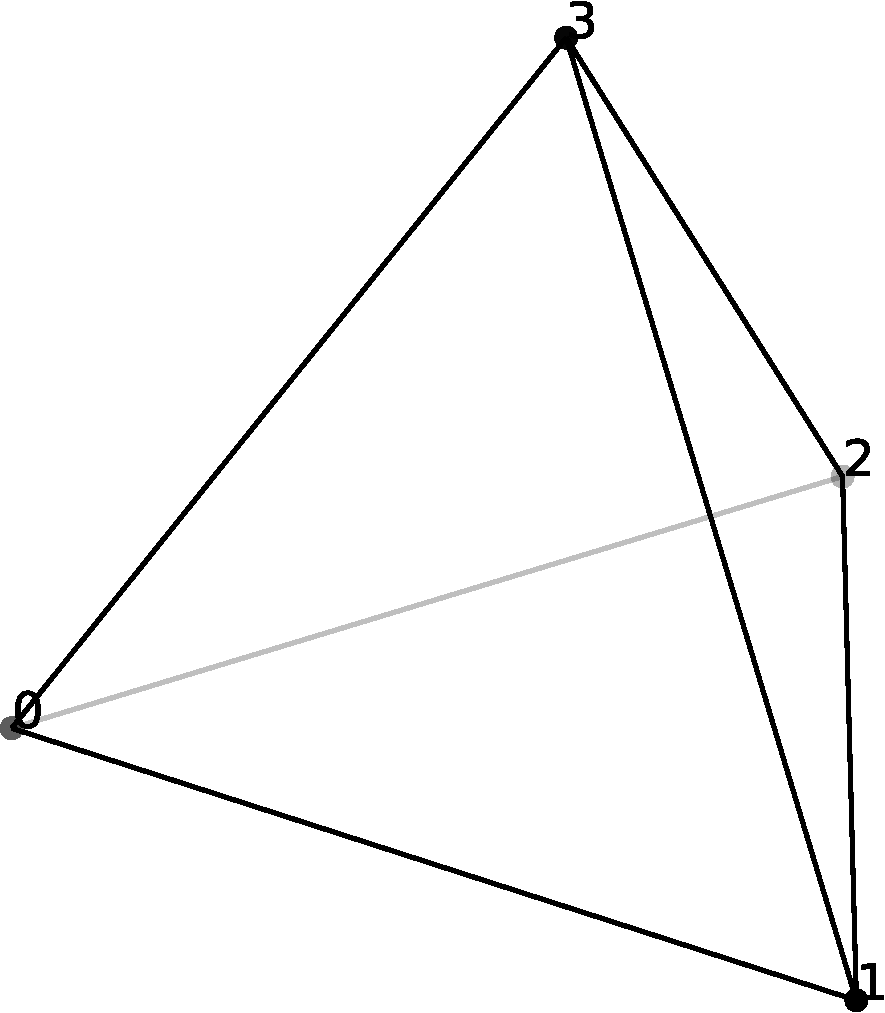
\includegraphics[scale=0.24]{../figures/tet.pdf}\qquad \qquad
    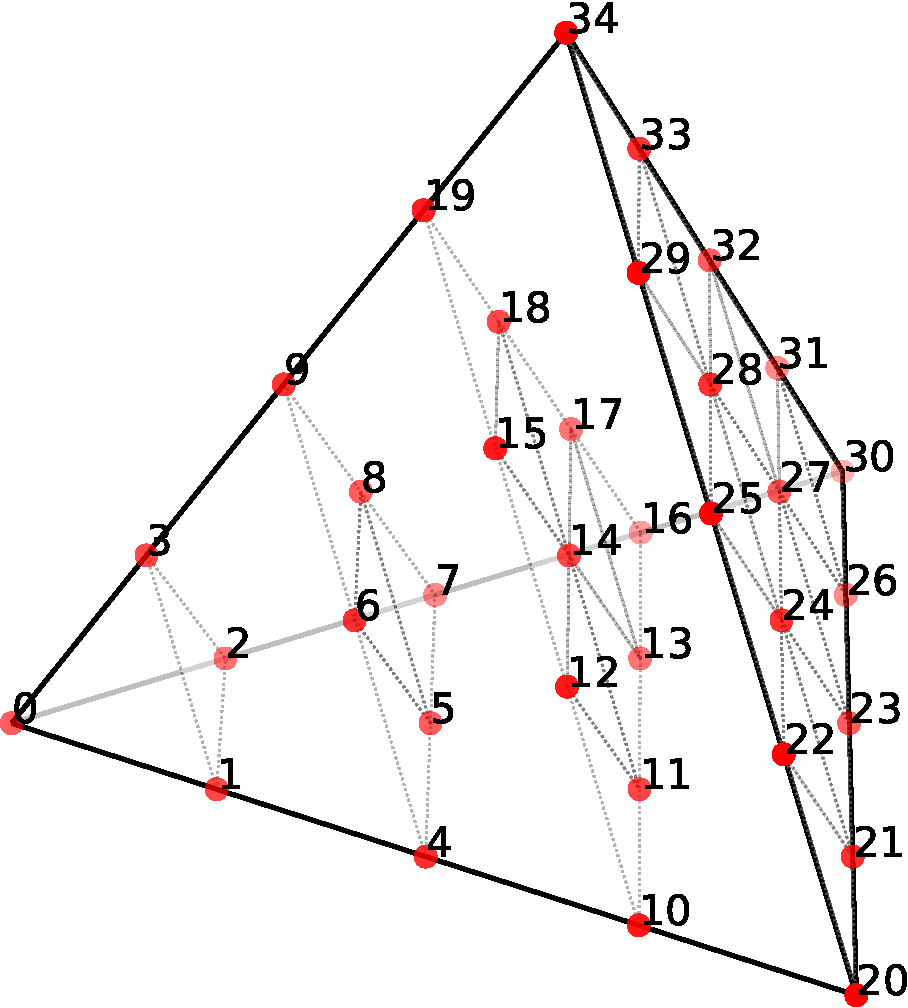
\includegraphics[scale=0.25]{../figures/tetdof4.pdf}
    \caption{Indexing rules for the vertices of a tetrahedron and interpolation points with \(k=4\) on it.}
    \label{fig:tet}
\end{figure}

\subsection{Lagrange finite element space}
Using the tetrahedral mesh as an illustrative example, Figure \ref{fig:tet} displays the local indexing rules for the tetrahedron's vertices and the interpolation points when \(k=4\). The tetrahedron's four vertices are ordered according to the right-hand rule, and the interpolation points adhere to the dictionary ordering map \(R_3(\boldsymbol \alpha)\). Since the Lagrange element is continuous, interpolation points on the boundary \(\partial T\) must have a global index. Thus, a unique index is required for points on vertices, edges, and faces, along with a mapping from local to global indices.

We begin by discussing the data structure of the tetrahedral mesh, denoted by \(\mathcal T_h\). Let the numbers of nodes, edges, faces, and cells in \(\mathcal T_h\) be represented as \lstinline{NN}, \lstinline{NE}, \lstinline{NF}, and \lstinline{NC}, respectively. We utilize two arrays to represent \(\mathcal T_h\):
\begin{itemize}
  \item \lstinline{node} (shape: \lstinline{(NN,3)}): \lstinline{node[i,j]} represents the $j$-th component of the Cartesian coordinate of the $i$-th vertex.
  \item \lstinline{cell} (shape: \lstinline{(NC,4)}): \lstinline{cell[i,j]} gives the global index of the $j$-th vertex of the $i$-th cell.
\end{itemize}
Given a tetrahedron denoted by \lstinline{[0,1,2,3]}, we define its local edges and faces as:
\begin{itemize}
  \item \lstinline{SEdge = [(0,1),(0,2),(0,3),(1,2),(1,3),(2,3)];}
  \item \lstinline{SFace = [(1,2,3),(0,2,3),(0,1,3),(0,1,2)];}
  \item \lstinline{OFace = [(1,2,3),(0,3,2),(0,1,3),(0,2,1)];}
\end{itemize}
Here, we introduced two types of local faces. The prefix \lstinline{S} implies sorting, and \lstinline{O} indicates outer normal direction. Both \lstinline{SFace[i,:]} and \lstinline{OFace[i,:]} represent the face opposite to the $i$-th vertex but with varied ordering. The normal direction as determined by the ordering of the three vertices of \lstinline{OFace} matches the outer normal direction of the tetrahedron. This ensures that the outer normal direction of a boundary \lstinline{face} points outward from the mesh. Meanwhile, \lstinline{SFace} aids in determining the global index of the interpolation points on the face. For an in-depth discourse on indexing, ordering, and orientation, we direct readers to \mc{sc3} in $i$FEM \cite{Chen.L2008c}.

Leveraging the \lstinline{unique} algorithm for arrays, we can derive the following arrays from \lstinline{cell}, \lstinline{SEdge}, and \lstinline{OFace}:
\begin{itemize}
  \item \lstinline{edge} (shape: \lstinline{(NE,2)}): \lstinline{edge[i,j]} gives the global index of the $j$-th vertex of the $i$-th edge.
  \item \lstinline{face} (shape: \lstinline{(NF,3)}): \lstinline{face[i,j]} provides the global index of the $j$-th vertex of the $i$-th face.
  \item \lstinline{cell2edge} (shape: \lstinline{(NC,6)}): \lstinline{cell2edge[i,j]} indicates the global index of the $j$-th edge of the $i$-th cell.
  \item \lstinline{cell2face} (shape: \lstinline{(NC,4)}): \lstinline{cell2face[i,j]} signifies the global index of the $j$-th face of the $i$-th cell.
\end{itemize}

Having constructed the edge and face arrays and linked cells to them, we next establish indexing rules for interpolation points on \(\mathcal T_h\). Let \(k\) be the degree of the Lagrange finite element space. The number of interpolation points on each cell is
\[
\mc{ldof} = \dim \mathbb P_k(T) = \frac{(k+1)(k+2)(k+3)}{6},
\]
and the total number on \(\mathcal T_h\) is
\[
\mc{gdof} = \mc{NN} + n_e^k \cdot \mc{NE} + n_f^k \cdot \mc{NF} + n_c^k \cdot \mc{NC},
\]
where
\[
n_e^k = k-1, \quad n_f^k = \frac{(k-2)(k-1)}{2}, \quad n_c^k = \frac{(k-3)(k-2)(k-1)}{6}.
\]
The global index of interpolation points on a face can be obtained via
\lstinline{SFace}, and the local index is derived from the dictionary ordering
map \(R_2(\boldsymbol \alpha)\) for \(0 \leq \alpha_i \leq k\). This mapping
guarantees that interpolation points on a face shared by two cells have the same
global index. Additionally, the global index of interpolation points inside a
cell is determined by the dictionary ordering map \(R_3(\boldsymbol \alpha)\).

In essence, establishing these rules facilitates the efficient assembly of
global matrices and vectors, which is crucial for computational efficiency.
Detailed algorithms are discussed in \cite{Chen.L2008c}.

\subsection{Constructing the \texttt{cell2ipoint} Array}
The two-dimensional array named \lstinline{cell2ipoint} of shape \lstinline{(NC,ldof)} is crucial in our discussion. For the $j$-th interpolation point of the $i$-th cell, we aim to determine its unique global index and store it in \lstinline{cell2ipoint[i,j]}.

The combination of the simplicial lattices set \(\mathbb T^n_k\) and the ordering map \(R(\boldsymbol \alpha)\) readily informs the position of each interpolation point relative to the simplex and its sub-simplexes. If the $j$-th interpolation point either coincides with a vertex or is situated inside a cell, the global indexing rule previously discussed simplifies the assignment of \lstinline{cell2ipoint[i,j]}. However, complications arise when the interpolation point is located within an edge or face since these elements can be shared by multiple cells.

Consider, for instance, the scenario where the $j$-th interpolation point lies within the $0$-th local face \(F_0\) of the $i$-th cell. Let \(\alpha = \) \lstinline{m = [m0,m1,m2,m3]} be its lattice point. Given that \(F_0\) is opposite to vertex $0$, we deduce that \(\lambda_0|_{F_0} = 0\), which implies \lstinline{m0} is 0. The remaining components of \(\boldsymbol m\) are non-zero, ensuring that the point is interior to \(F_0\). Using the dictionary ordering, we express \(j\) as:

\begin{align*}
j =& \frac{(\mc{m1} + \mc{m2} + \mc{m3})(\mc{m1} + \mc{m2} + \mc{m3} + 1)(\mc{m1} + \mc{m2} + \mc{m3} + 2)}{6} \\
&+ \frac{(\mc{m2} + \mc{m3})(\mc{m2} + \mc{m3} + 1)}{2} + \mc{m3}.
\end{align*}

Two representations for the face with global index \lstinline{cell2face[i,0]} are subsequently acquired:

\begin{itemize}
  \item \lstinline{LFace = cell[i,SFace[0,:]]} (local representation)
  \item \lstinline{GFace = face[cell2face[i,0],:]} (global representation)
\end{itemize}

Although \lstinline{LFace} and \lstinline{GFace} comprise identical vertex numbers, their ordering differs. The array \lstinline{m = [m1,m2,m3]} has a one-to-one correspondence with the vertices of \lstinline{LFace}. To match this array with the vertices of \lstinline{GFace}, a reordering based on argument sorting is performed:

\begin{lstlisting}
i0 = argsort(argsort(GFace));
i1 = argsort(LFace);
i2 = i1[i0];
m = m[i2].
\end{lstlisting}

From the reordered \lstinline{m = [m1,m2,m3]}, the local index \(\ell\) of the $j$-th interpolation point on the global face \lstinline{f = cell2face[i,0]} can be deduced:

\begin{align*}
   \ell = & \frac{(\mc{m2}-1 + \mc{m3}-1)(\mc{m2}-1 + \mc{m3}-1 + 1)}{2} + \mc{m3}-1 \\
   =& \frac{(\mc{m2} + \mc{m3} -2)(\mc{m2} + \mc{m3} - 1)}{2} + \mc{m3}-1.
\end{align*}

It's worth noting that the index of interpolation points solely within the face needs consideration. Finally, the global index \(J\) for the $j$-th interpolation point within the $0$-th local face of the $i$-th cell is:

\[
J = \mc{NN} + n_e^k\cdot \mc{NE} + n_f^k\cdot \mc{NF} + \ell.
\]

In conclusion, we've elucidated the construction of global indexing for interpolation points inside cell faces. This method can be generalized for edges and, more broadly, for interior interpolation points of the low-dimensional sub-simplex of an \(n\)-dimensional simplex.

\end{document}

